\documentclass{article}
\usepackage[utf8]{inputenc}
\usepackage{amsmath}
\usepackage{amssymb}
\usepackage{graphicx}

\begin{document}
\section*{Estimating a Tridiagonal Matrix}
We are given two vectors $\mathbf{z}, \mathbf{c} \in \mathbb{R}^{n}$, $n > 2 \in \mathbb{N}$ of measured values. The two real values $\alpha^{*}$ and $\beta^{*}$ are defined as
\begin{equation*}
    \left(\alpha^{*}, \beta^{*}\right) = \underset{\alpha,\beta \in \mathbb{R}}{\text{argmin}} \left\lVert \mathbf{T}_{\alpha, \beta}\mathbf{z} - \mathbf{c}\right\rVert
\end{equation*}
where $\mathbf{T}_{\alpha, \beta} \in \mathbb{R}^{n \times n}$ is the following \textbf{tridiagonal matrix}
\begin{equation*}
    \mathbf{T}_{\alpha,\beta} = \begin{bmatrix}
    \alpha & \beta & 0 & \dots & 0  \\
    \beta & \alpha & \beta & \ddots & \vdots \\
    0 & \beta & \ddots & \ddots & 0 \\
    \vdots & \ddots & \ddots & \alpha & \beta \\
    0 & \dots & 0 & \beta & \alpha
    \end{bmatrix}
\end{equation*}
Let us look at an example for $\mathbf{T}_{\alpha, \beta}\mathbf{z}$.
\begin{equation*}  \mathbf{T}_{\alpha,\beta} = \begin{bmatrix}
    \alpha & \beta & 0 & 0 & 0 \\
    \beta & \alpha & \beta & 0 & 0 \\
    0 & \beta & \alpha & \beta & 0 \\
    0 & 0 & \beta & \alpha & \beta \\
    0 & 0 & 0 & \beta & \alpha
    \end{bmatrix}
    \begin{bmatrix}
        z_{1} \\
        z_{2} \\
        z_{3} \\
        z_{4} \\
        z_{5}
    \end{bmatrix}
    = 
    \begin{bmatrix}
        \alpha z_{1} + \beta z_{2} \\
        \beta z_{1} + \alpha z_{2} + \beta z_{3} \\
        \beta z_{2} + \alpha z_{3} + \beta z_{4} \\
        \beta z_{3} + \alpha z_{4} + \beta z_{5} \\
        \beta z_{4} + \alpha z_{5}
    \end{bmatrix} = 
    \begin{bmatrix}
        \alpha z_{1} + \beta z_{2} \\
        \alpha z_{2} + \beta \left(z_{1} +z_{3}\right) \\
        \alpha z_{3} + \beta\left(z_{2} + z_{3}\right) \\
        \alpha z_{4} + \beta \left(z_{3} + z_{5}\right) \\
        \alpha z_{5} +\beta z_{4}
    \end{bmatrix}
\end{equation*}
This leads to the modified system
\begin{equation*}
   \begin{bmatrix}
        \alpha z_{1} + \beta z_{2} \\
        \alpha z_{2} + \beta \left(z_{1} +z_{3}\right) \\
        \alpha z_{3} + \beta\left(z_{2} + z_{3}\right) \\
        \alpha z_{4} + \beta \left(z_{3} + z_{5}\right) \\
        \alpha z_{5} +\beta z_{4}
    \end{bmatrix} = 
    \begin{bmatrix}
        z_{1} & z_{2} \\
        z_{2} & z_{1} +z_{3} \\
        z_{3} & z_{2} + z_{4} \\
        z_{4} & z_{3} + z_{5} \\
        z_{5} & z_{4}
    \end{bmatrix}
     \begin{bmatrix}
         \alpha \\
         \beta
     \end{bmatrix}=: \mathbf{A}\mathbf{x}
\end{equation*}
We hence define the linear least squares problem 
\begin{equation*}
    \mathbf{x}^{*} = \underset{x\in\mathbb{R}^{2}}{\left\lVert \mathbf{A}\mathbf{x} - \mathbf{b}\right\rVert_{2}}
\end{equation*}
for $\mathbf{A} \in \mathbb{R}^{n,2}$, $\mathbf{x}\in \mathbb{R}^{2}$ and $\mathbf{b}\in \mathbb{R}^{n}$ with
\begin{equation*}
    \mathbf{A} = \begin{bmatrix}
        z_{1} & z_{2} \\
         z_{2} & z_{1} +z_{3} \\
         \vdots & \vdots \\
         z_{n-1} & z_{n-2} + z_{n} \\
         z_{n} & z_{n-1}
    \end{bmatrix} \quad
    \mathbf{x} = \begin{bmatrix}
        \alpha \\
        \beta
    \end{bmatrix}
    \quad 
    \mathbf{b} = \mathbf{c}
\end{equation*}

\pagebreak

\subsection*{3-2.b}
We are tasked with stating the \textbf{normal equations} associated with the above linear least squares problem. They are given by
\begin{equation*}
    \mathbf{A}^{\mathsf{T}}\mathbf{A}\mathbf{x} = \mathbf{A}^{\mathsf{T}}\mathbf{c}
\end{equation*}
Computing this gives us
\begin{align*}
   \mathbf{A}^{\mathsf{T}}\mathbf{A} &=  
   \begin{bmatrix}
        z_{1} & z_{2} & \dots & z_{n-1} & z_{n} \\
        z_{2} & z_{1} + z_{3} & \dots& z_{n-2} + z_{n} & z_{n-1}
    \end{bmatrix}
   \begin{bmatrix}
        z_{1} & z_{2} \\
         z_{2} & z_{1} +z_{3} \\
         \vdots & \vdots \\
         z_{n-1} & z_{n-2} + z_{n} \\
         z_{n} & z_{n-1}
    \end{bmatrix} \\
    &= 
    \begin{bmatrix}
        \sum_{i=1}^{n}z_{i}^{2} & \sum_{i =2}^{n-1}z_{i}\left(z_{i-1} + z_{i+1}\right) + z_{1}z_{2} + z_{n}z_{n-1} \\[1mm]
        \sum_{i =2}^{n-1}z_{i}\left(z_{i-1} + z_{i+1}\right) + z_{1}z_{2} + z_{n}z_{n-1} & \sum_{i=2}^{n-1}\left(z_{i-1} +  z_{i + 1}\right)^{2} + z_{2}^{2} + z_{n-1}^{2}
    \end{bmatrix}
\end{align*}
\noindent Let us take a closer look at the term
\begin{align*}
\left(\mathbf{A}^{\mathsf{T}}\mathbf{A}\right)_{1,2} &=  
    \sum_{i =2}^{n-1}z_{i}\left(z_{i-1} + z_{i+1}\right) + z_{1}z_{2} + z_{n}z_{n-1} \\
    &= \left(z_{2}z_{1} + z_{2}z_{3}\right) +\left(z_{3}z_{2} + z_{3}z_{4}\right) + \dots + \left(z_{n-1}z_{n-2} + z_{n-1}z_{n}\right) + z_{1}z_{2} + z_{n}z_{n-1} \\
    &=\left(z_{1}z_{2} + z_{2}z_{3}\right) +\left(z_{2}z_{3} + z_{3}z_{4}\right) + \dots + \left(z_{n-2}z_{n-1} + z_{n-1}z_{n}\right) + z_{1}z_{2} + z_{n-1}z_{n} \\
    &=z_{1}z_{2}  +
    \left(z_{1}z_{2} + z_{2}z_{3}\right) +\left(z_{2}z_{3} + z_{3}z_{4}\right) + \dots + \left(z_{n-2}z_{n-1} + z_{n-1}z_{n}\right) +  z_{n-1}z_{n} \\
    &= \left(z_{1}z_{2}  +
    z_{1}z_{2}\right) + \left(z_{2}z_{3} + z_{2}z_{3}\right) + \dots + \left(z_{n-2}z_{n-1} + z_{n-2}z_{n-1}\right) +  \left(z_{n-1}z_{n} 
 + z_{n-1}z_{n} \right)\\
 &= 2\sum_{i=1}^{n-1}z_{i}z_{i+1}
\end{align*}

Let us next look at the bottom right term
\begin{align*}
    \left(\mathbf{A}^{\mathsf{T}}\mathbf{A}\right)_{2,2} &= \sum_{i=2}^{n-1}\left(z_{i-1} +  z_{i + 1}\right)^{2} + z_{2}^{2} + z_{n-1}^{2} \\
    &= \left(z_{1} + z_{3}\right)^{2} + \dots + \left(z_{n-2}+z_{n}\right)^{2} + z_{2}^{2} + z_{n-1}^{2} \\
    &= \left(z_{1}^{2} + 2z_{1}z_{3} + z_{3}^{2}\right) + \dots + \left(z_{n-2}^{2} + 2z_{n-2}z_{n}+z_n^{2}\right) + z_{2}^{2} + z_{n-1}^{2} \\
    &= z_{1}^{2} + z_{2}^{2}+ 2z_{3}^{2}  + \dots + 2z_{n-2}^{2} + z_{n-1}^{2} + 2z_{1}z_{3} + \dots 2z_{n-2}z_{n} + z_{2}^{2} + z_{n-1}^{2} \\
    &= z_{1}^{2} + 2\sum_{i=2}^{n-1}\left(z_{i}^{2} +z_{i-1}z_{i+1}\right) + z_{n}^{2}
\end{align*}
This results in the following matrix.
\begin{equation*}
    \mathbf{A}^{\mathsf{T}}\mathbf{A} = 
    \begin{bmatrix}
        \sum_{i=1}^{n}z_{i}^{2} & 2\sum_{i=1}^{n-1}z_{i}z_{i+1} \\[1mm]
        2\sum_{i=1}^{n-1}z_{i}z_{i+1} & z_{1}^{2} + 2 \sum_{i=2}^{n-1}\left(z_{i}^{2}+z_{i}z_{i+1}\right) + z_{n}^{2}
        
    \end{bmatrix}
\end{equation*}

\pagebreak

\subsection*{3-2.c}
We are now tasked with implementing a \verb|C++| function \verb|lsqEst| that computes the optimal (in least-squares sense) parameters $\alpha^{*}$ and $\beta^{*}$ from data vectors \verb|z| and \verb|c| (using the method of normal equations). Looking through the lecture document we spot this piece of code.

\begin{figure}[!hbt]
    \centering
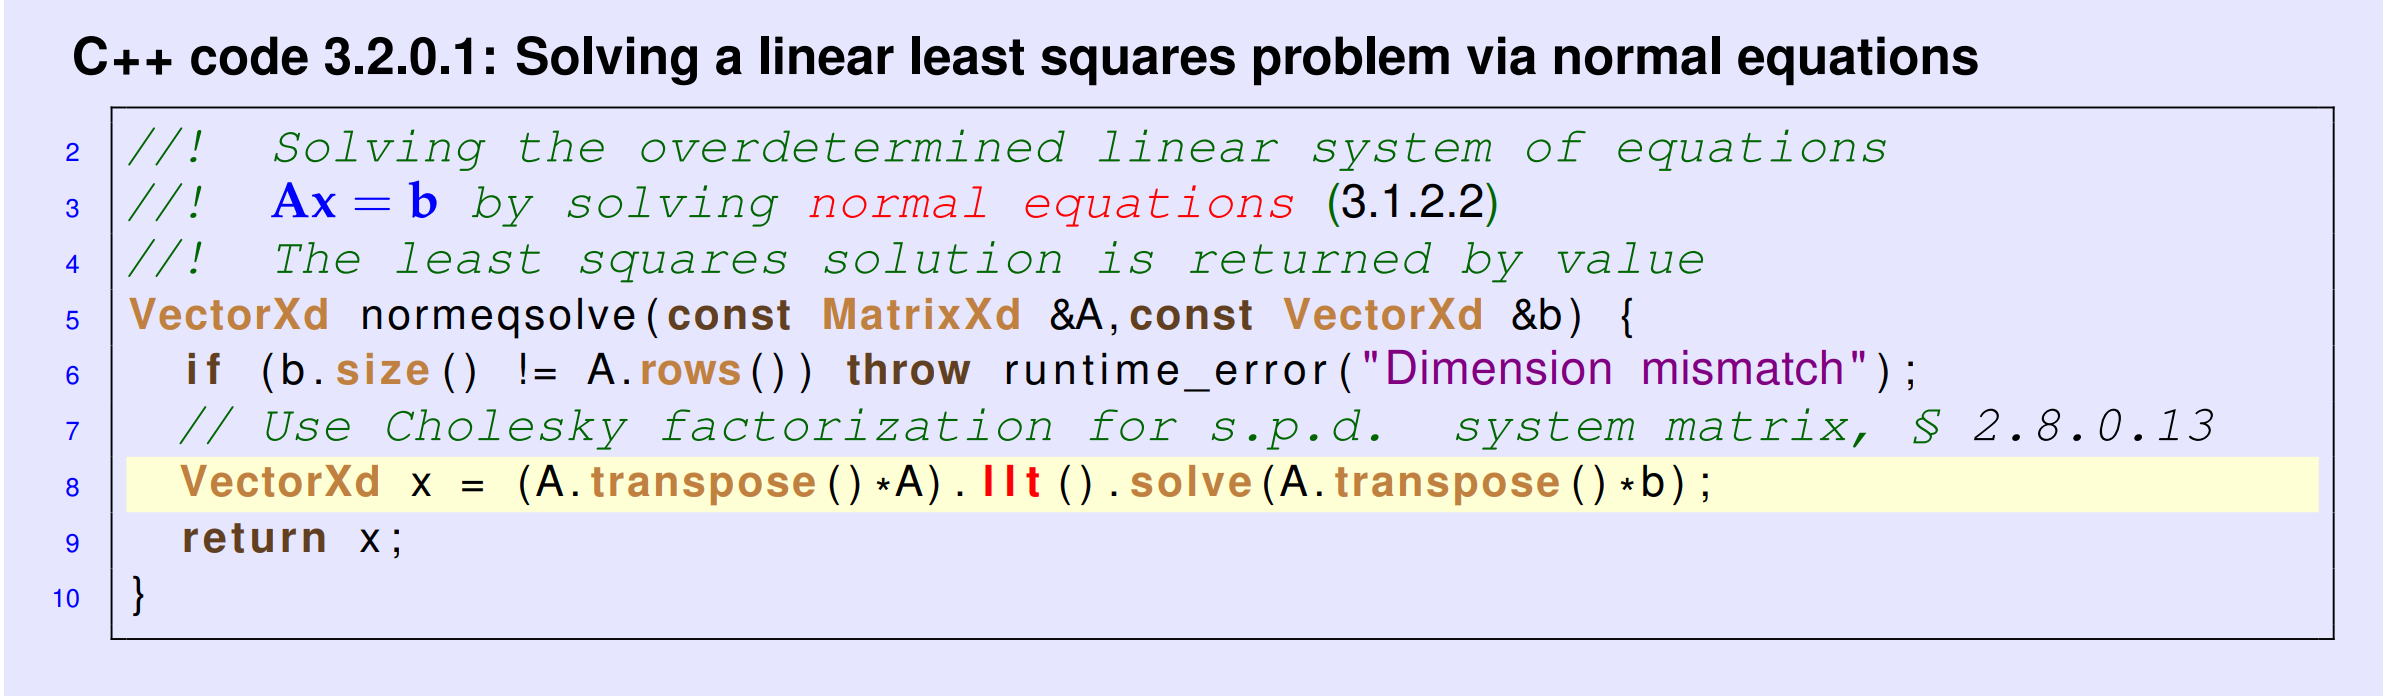
\includegraphics[width=1.0\linewidth]{NormalEquationsLinearLeastSquares.png}
\end{figure}
Here we use the Cholesky decomposition (not really discussed in the lecture) to decompose $\mathbf{A}^{\mathsf{T}}\mathbf{A}$, which uses that this matrix is symmetric positive definite. We are left with constructing the matrix $\mathbf{A}^{\mathsf{T}}\mathbf{A}$, which we do given the above structure. This produces the following code.

\begin{figure}[!hbt]
    \centering
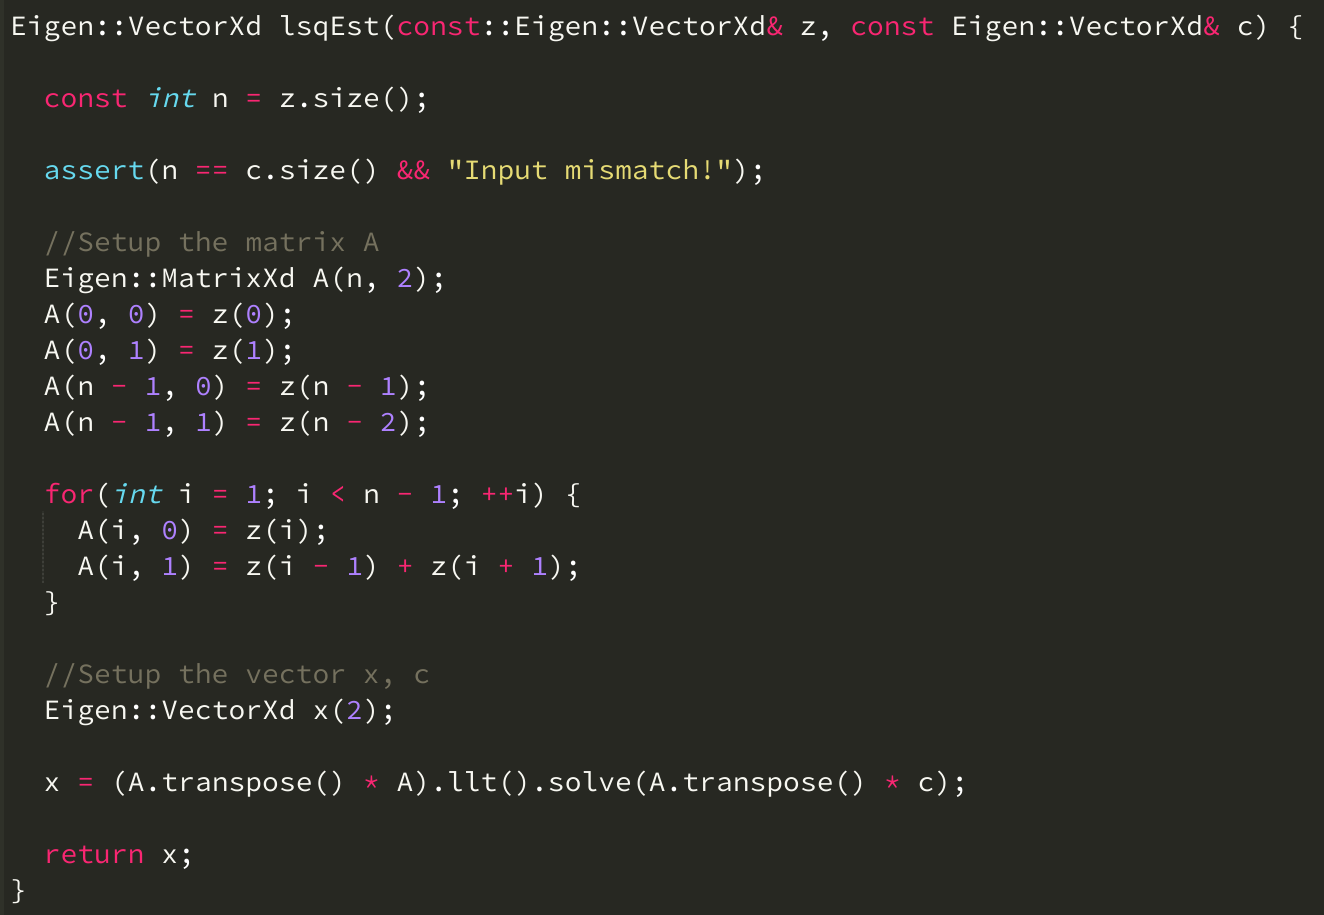
\includegraphics[width=1.0\linewidth]{3-2.c.png}
\end{figure}
\end{document}
